% ----------
% A LaTeX template for course project reports
% 
% This template is modified from "Tech Report ala MIT AI Lab (1981)"
% 
% ----------
\documentclass[12pt, letterpaper, twoside]{article}
\usepackage{geometry}
\usepackage[utf8]{inputenc}
\usepackage[english]{babel}
\usepackage[runin]{abstract}
\usepackage{titling}
\usepackage{booktabs}
\usepackage{fancyhdr}
\usepackage{helvet}
\usepackage{csquotes}
\usepackage{graphicx}
\usepackage{blindtext}
\usepackage{parskip}
\usepackage{etoolbox}
\usepackage{float}

\input{preamble.tex}

% ----------
% Variables
% ----------

\title{\textbf{{\LARGE Assignment \#03 — Smart Tank Monitoring System}} \\ {\ Embedded Systems and Internet of Things Course}} % Full title of your tech report
\runningtitle{Ass. \#03 — SMTS} % Short title
\author{Nicholas Magi \\ \texttt{0001113915} \and Rebecca Scarcelli \\ \texttt{0001118585} \and Elettra Ventura \\ \texttt{0001117272}} % Full list of authors
\runningauthor{N. Magi, R. Scarcelli, E. Ventura} % Short list of authors
\affiliation{University of Bologna, Cesena Campus} % Affiliation e.g. University or Company
\department{Department of Computer Science and Engineering} % Department or Office
\theyear{2026} % year of the tech report
\mydate{February 3, 2026} %the date


% ----------
% actual document
% ----------
\begin{document}
\maketitle

\begin{abstract}
    The project requires a 4-tier IoT system to monitor rainwater levels and control a drainage valve. A PC back-end coordinates an ESP32 sensor, Arduino valve controller, and web dashboard via MQTT, HTTP, and Serial. It automates drainage based on specific water thresholds but allows local or remote manual overrides. Deliverables include FSM-based code for all subsystems and a technical report with schematics and a video demo.
\end{abstract}

\vspace{2.5cm}

% Uncomment the following to add thanks.
% {\footnotesize
%     \noindent
%     Special thanks to \textbf{Person 1} and \textbf{Affiliation A} for financial support for this project.
% }

\thispagestyle{firstpage}

\pagebreak

% ----------
% End of first page
% ----------

\newgeometry{} % Redefine geometries (normal margins)

\tableofcontents

\pagebreak

\section{Introduction}
\label{sec:intro}

\subsection{Requirements — v1.0.0-20251112}
 
We want to realise an IoT system monitoring the rainwater level of a tank.  The system is composed of 4 subsystems: 

\begin{figure}[htbp]
\centering

\includegraphics[width=\textwidth]{assets/imgs/assignment-03-sketch.png}
\caption{System's simplified architecture diagram}
\end{figure}

\subsubsection*{Description}

\paragraph*{Components}

The system is composed by four subsystems:

\begin{itemize}
    \item \textbf{Tank Monitoring subsystem (TMS)} - based on ESP
    \begin{itemize}
        \item embedded system to monitor the rainwater level in the tank
        \item It interacts with the Control Room subsystem (CUS) via MQTT
    \end{itemize}
    \item \textbf{Control Unit subsystem (CUS)}  - Back-end, running on a PC 
    \begin{itemize}
        \item main subsystem, governing and coordinating  the whole system
        \item It interacts via MQTT with the Tank Monitoring Subsystem (TMS)  
        \item It interacts through the serial line with the Water Channels Subsystem (WCS)  
        \item It interacts via HTTP with the Dashboard Subsystem (DBS) 
    \end{itemize}
    \item \textbf{Water Channel Subsystem (WCS)} - based on Arduino
    \begin{itemize}
        \item Embedded system controlling the water channel connecting the tank with the water channel network. 
        \item It interacts via serial line with the Control Unit Subsystem (CUS).
        \item It provides a panel for human operators to interact in place.
    \end{itemize}
    \item \textbf{Dashboard subsystem (DBS)} - Frontend/web app, running on the PC or any device
    \begin{itemize}
        \item Front-end for remote operators to visualise data and interact with the system.
        \item it interacts via HTTP with the Control Unit Subsystem.
    \end{itemize}
\end{itemize}

\paragraph*{Hardware components}

\begin{itemize}
    \item \textbf{TMS}
    \begin{itemize}
        \item SoC ESP32 board (or ESP8266) including:
        \item 1 sonar
        \item 1 green led 
        \item 1 red led
    \end{itemize}
    \item \textbf{WCS}
    \begin{itemize}
        \item Microcontroller Arduino UNO board including:
        \item 1 servo motor
        \item 1 potentiometer
        \item 1 tactile button
        \item 1 LCD display
    \end{itemize}
\end{itemize}


\paragraph*{Description of the behaviour}

The system is meant to monitor the rainwater level inside the tank, and - depending on values - controlling the opening of a water channel connecting the tank to a network of water channers.   The overall system can be in two different modes: \texttt{AUTOMATIC} or \texttt{MANUAL}. In \texttt{AUTOMATIC} mode, the system automatically controls the opening of the water channel, depending on the current rainwater level in the tank. In \texttt{MANUAL} mode, the opening is controlled manually by an operator. The starting mode when booting is \texttt{AUTOMATIC}. 

\textit{Details}

\begin{itemize}
    \item The \textbf{TMS} is responsible for continuously monitoring the level of the rainwater level, by means of proper sensors (e.g. a sonar). 
    \begin{itemize}
        \item The rainwater level are sampled at frequency F and sent to the \textbf{CUS} subsystem.
        \item When the system is working correctly (network ok, sending data ok)  the green led is on and the red is off; otherwise -- in the case of network problems -- the red led should be on and the green led off.
    \end{itemize}
    \item The \textbf{WCS} subsystem is responsible for controlling a valve (with a motor) opening/closing a water channel draining water from the tank to the water channel network.
    \begin{itemize}
        \item The opening range is in percentage: from 0\% = channel closed (motor position 0 degree), up to 100\% = channel full open (motor position 90$^\circ$ degree).
        \item The water channel opening level depends on the state of the system, established by the \textbf{CUS} subsystem (see later). 
        \item The \textbf{WCS} includes a button to enable the \texttt{MANUAL} mode, in particular:
        \begin{itemize}
            \item When the button is pressed, the system enters in \texttt{MANUAL} mode, so that the water channel opening level can be manually controlled by operators using a potentiometer. 
            \item To exit from the \texttt{MANUAL} model, the button must be pressed again.  
        \end{itemize}
        \item The \textbf{WCS} subsystem is equipped also with an LCD display reporting: 
        \begin{itemize}
            \item the current valve opening level of the water channel.
            \item the current mode (\texttt{AUTOMATIC} or \texttt{MANUAL}), or \texttt{UNCONNECTED} (see later).
        \end{itemize}
    \end{itemize}
    \item The \textbf{CUS} subsystem is in charge of the policy governing the behaviour of the system. In particular:
    \begin{itemize}
        \item Rainwater level monitoring
        \begin{itemize}
            \item When the rainwater level exceeds the level $L_1$ (but below $L_2$, with $L_1 < L_2$) for more than $T_1$ time, the water channel is opened at 50\% until the rainwater level is below $L_1$.
            \item If the the rainwater level exceeds the level $L_2$, the water channel is immediately opened at 100\%, until the value is below $L_2$.
        \end{itemize}
    \end{itemize}
\end{itemize}

If the \textbf{CUS} is not receiving data for more than $T_2$  time units from the \textbf{TMS} (because of network problems), then the system enters into an \texttt{UNCONNECTED} state, which is restored to a normal state only if/when the network problems are solved.

\begin{itemize}
    \item The \textbf{DBS} subsystem is a dashboard for visualising the state of the Tank Monitoring system, including:
    \begin{itemize}
        \item A graph of the rainwater level, considering the last N measurements.
        \item The current value of the valve opening percentage.
        \item The state of the system:  \texttt{MANUAL}, \texttt{AUTOMATIC}, \texttt{UNCONNECTED} or \texttt{NOT AVAILABLE}. 
        \begin{itemize}
            \item the state is labelled as \texttt{NOT AVAILABLE} when the \textbf{CUS} is not reachable, for any reason.
        \end{itemize}
    \end{itemize}
\end{itemize}
    
Besides, it includes: 
\begin{itemize}
    \item a GUI button to switch the modality (\texttt{MANUAL}, \texttt{AUTOMATIC}).
    \item a GUI widget to control the opening level of the valve in the \textbf{WCS} (when in \texttt{MANUAL} mode).
\end{itemize}


\subsubsection*{The assignment}

Design and develop a prototype of the Tank Monitoring system, considering as further  requirements:
\begin{itemize}
    \item About the \textbf{TMS} subsystem:
    \begin{itemize}
        \item it must run on an ESP32 (or an equivalent SoC board).
        \item The control logic must be designed and implemented using finite state machines (synchronous or asynchronous) and (possibly, if useful) task-based architectures, exploiting the RTOS.
        \item Must use MQTT to communicate with the \textbf{CUS} subsystem.
    \end{itemize}
    \item About the \textbf{WCS} subsystem:
    \begin{itemize}
        \item It must run on an Arduino (or an equivalent MCU board).
        \item The control logic must be designed and implemented using finite state machines (synchronous or asynchronous) and  (possibly, if useful) task-based architectures.
        \item It must communicate with the \textbf{CUS} subsystem via serial line.
    \end{itemize}
    \item About the \textbf{CUS} subsystem: 
    \begin{itemize}
        \item It must run on a PC, as a server/back-end.
        \item No specific constraints about the programming/sw technology to be used.
        \item It must use:
        \begin{itemize}
            \item MQTT to communicate with the \textbf{TMS} subsystem.
            \item HTTP to communicate  with the \textbf{DBS} subsystem. 
            \item the serial line to interact with the \textbf{WCS}.
        \end{itemize}
    \end{itemize}
    \item About the \textbf{DBS} subsystem
    \begin{itemize}
        \item It must run on a PC
        \item No specific constraints about the programming/sw technology to be used.
        \item It must use HTTP to interact with the \textbf{CUS} subsystem.
    \end{itemize}
\end{itemize}

For any aspect not specified, you are free to choose the approach you consider more useful or valuable.

\textbf{The Deliverable}

The deliverable consists in a zipped folder assignment-03.zip including 4 subdirectories - one for each subsystem: \texttt{tms},\texttt{cus}, \texttt{wcs},\texttt{DBS}) - and a \texttt{doc} subdirectory, including the report. The report must be in PDF or MD (\texttt{report.pdf} or \texttt{report.md}) must include a high-level description of the behaviour of subsystems (using FSMs), a representation of the schema/breadboard and the link to a short video demonstrating the system.


\section{System Architecture - Control Unit Subsystem (CUS)}

\begin{figure}[htbp]
\centering
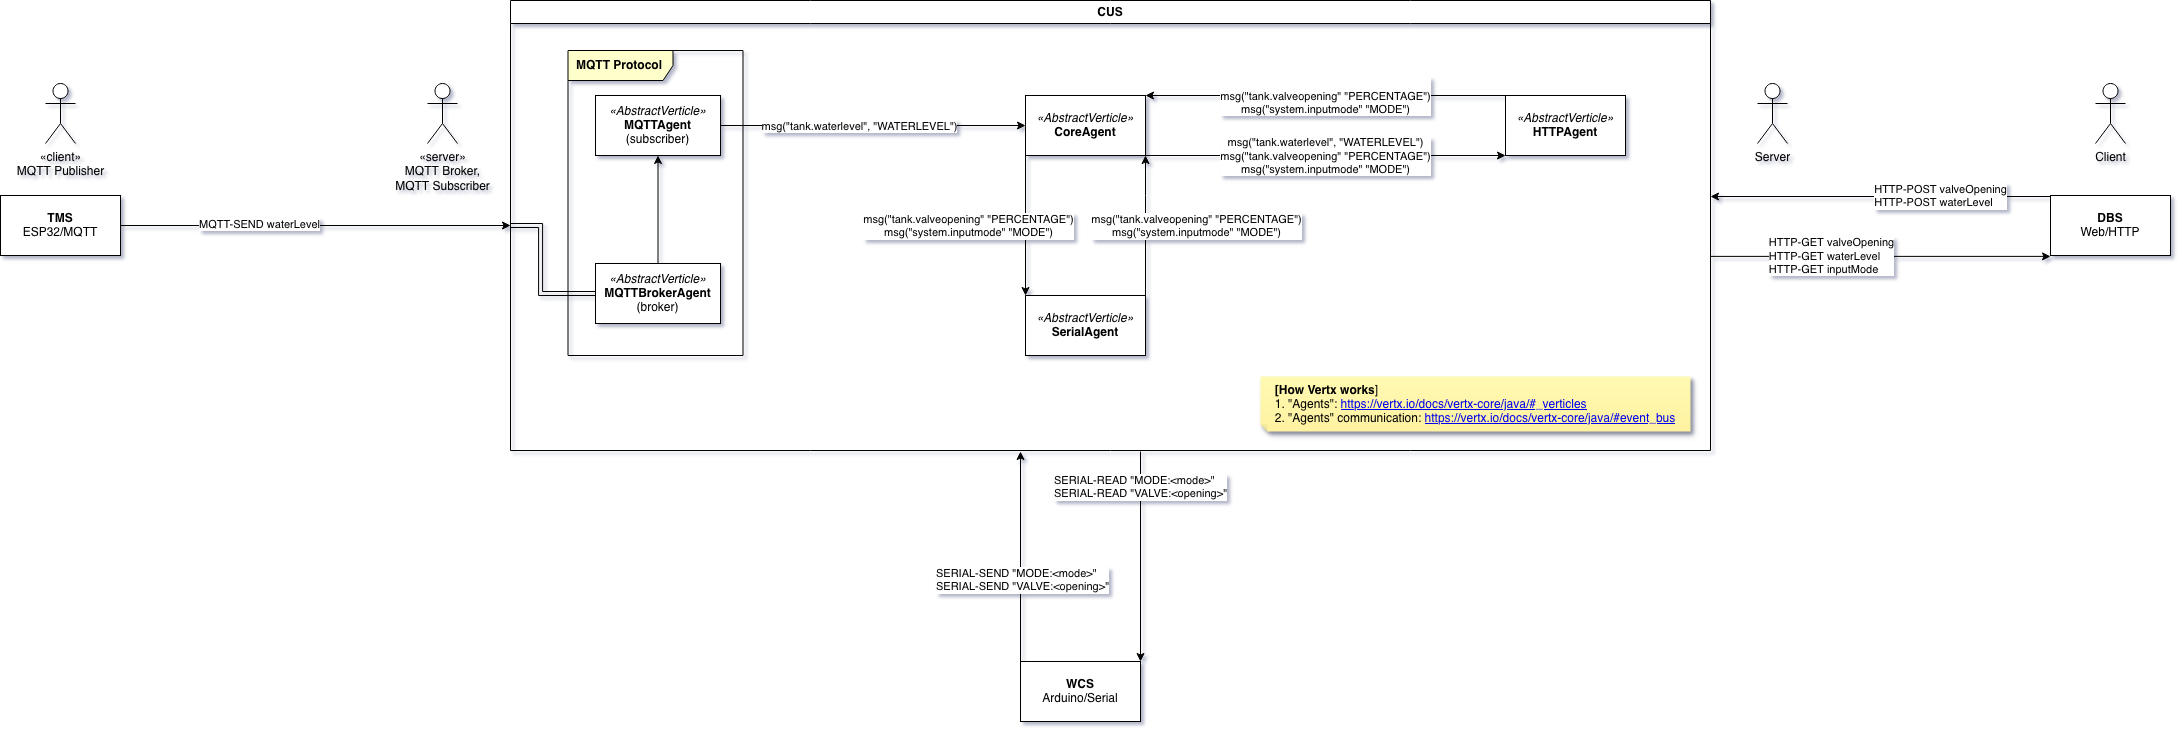
\includegraphics[width=\linewidth]{assets/imgs/CUS-Architecture-Diagram.drawio.png}
\caption{System architecture}
\end{figure}

The core of the whole system is the CUS: \textbf{Control Unit Subsystem}. It is the nevralgic center of the communication, and contains the logic responsible in opening and closing the valve when the system is in \verb|AUTOMATIC| mode and the water levels reach certain thresholds. 

\subsection{Implementation}
The system is written in Java, and the \verb|vertx| library has been used to implement internally all the \textbf{agents} (\verb|verticles|) needed to interact with all the different protocols involved.

In particular, we have:
\begin{enumerate}
    \item \verb|CoreAgent|: contains the previously described logic, implemented using some timers;
    \item \verb|HttpAgent|: acts like a small HTTP server and provides all the API endpoints required by the DBS to send/receive the data;
    \item \verb|SerialAgent|: interface to WCS; it manages serial communication;
    \item \verb|MqttBroker|: serves like an embedded MQTT broker that manages client connections and handles the data stream from the TMS via the vertx-mqtt library;
    \item \verb|MqttAgent|: the MQTT client that is subscribed to \verb|tank/waterlevel| topic and constantly receives sampled values from TMS. 
\end{enumerate}

\section{Water Channel Subsystem - (WCS)}

\begin{figure}[H]
\centering
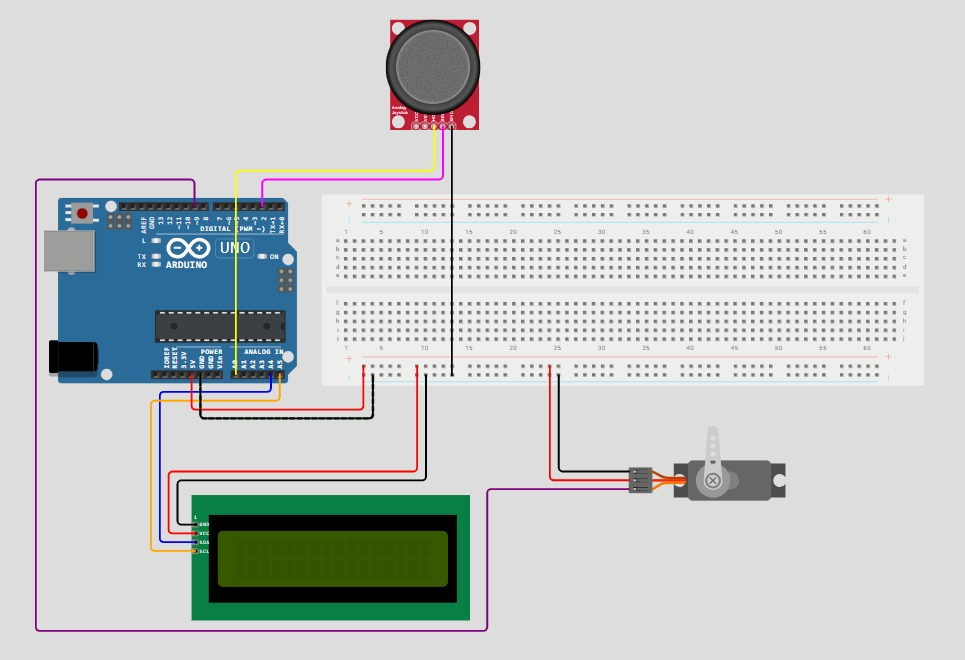
\includegraphics[width=\linewidth]{assets/imgs/WCS-Circuit.jpeg}
\caption{Subsystem circuit.}
\end{figure}

\begin{figure}[H]
\centering
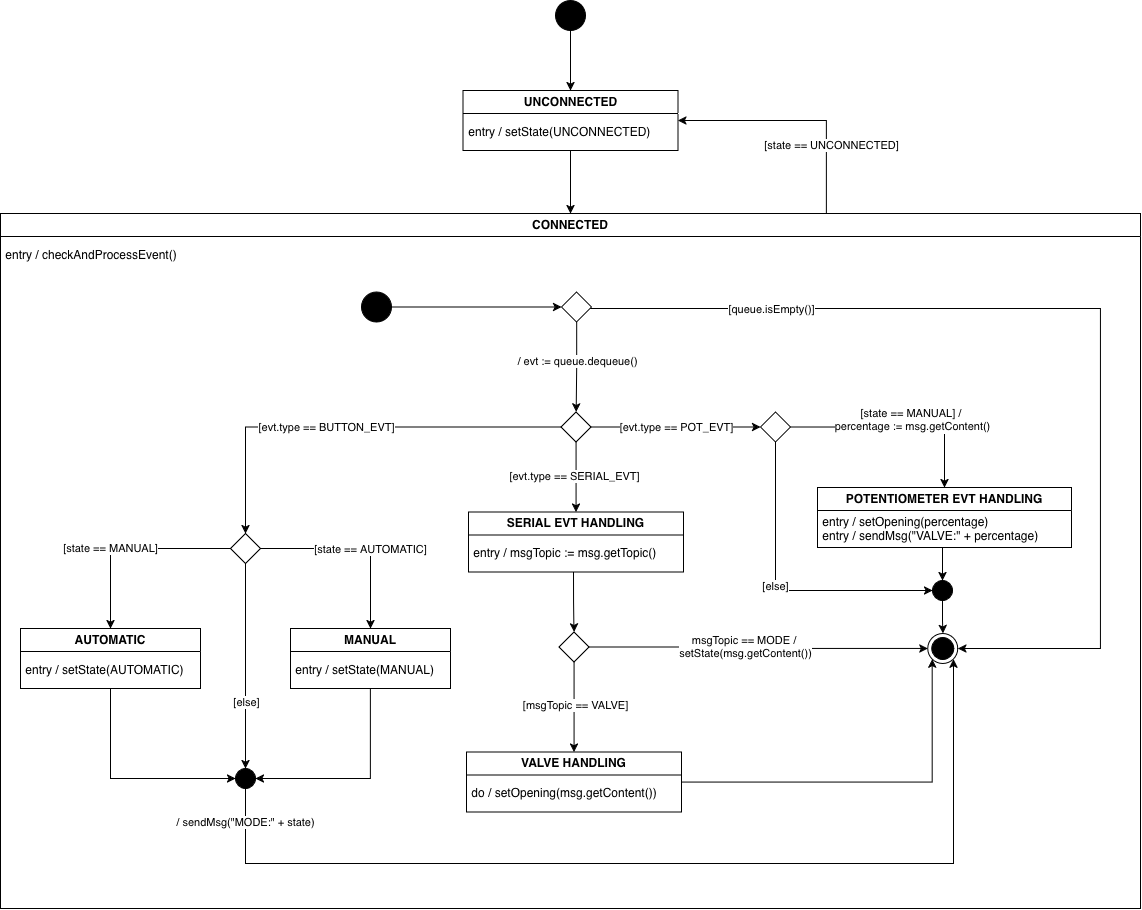
\includegraphics[width=\linewidth]{assets/imgs/WCS-Async-FSM.drawio.png}
\caption{Subsystem asynchronous FSM diagram}
\label{fig:asyncFSM}
\end{figure}

\subsection{Implementation}

The Water Channel Subsystem's behaviour, by its definition from the requirements, is driven by many events: as described by the Fig. \ref{fig:asyncFSM}, we identified three types of them:
\begin{itemize}
    \item \verb|ButtonEvent| happens via interrupts when the button is clicked, and it can toggle the system state to either \verb|AUTOMATIC| or \verb|MANUAL|;
    \item \verb|SerialEvent| is fired whenever a message is received from the Serial bus: messages regarding the input mode of the system or the opening of the valve; 
    \item \verb|PotentiometerEvent| tells that the potentiometer acting as a lever has changed, so the valve should open accordingly (if the system is in \verb|MANUAL| mode);
\end{itemize}

The events processing is handled by the class \verb|AsyncFSM|, which reads events via \textbf{polling} from the shared \textbf{event queue} and acts consequently.

\begin{figure}[H]
\centering
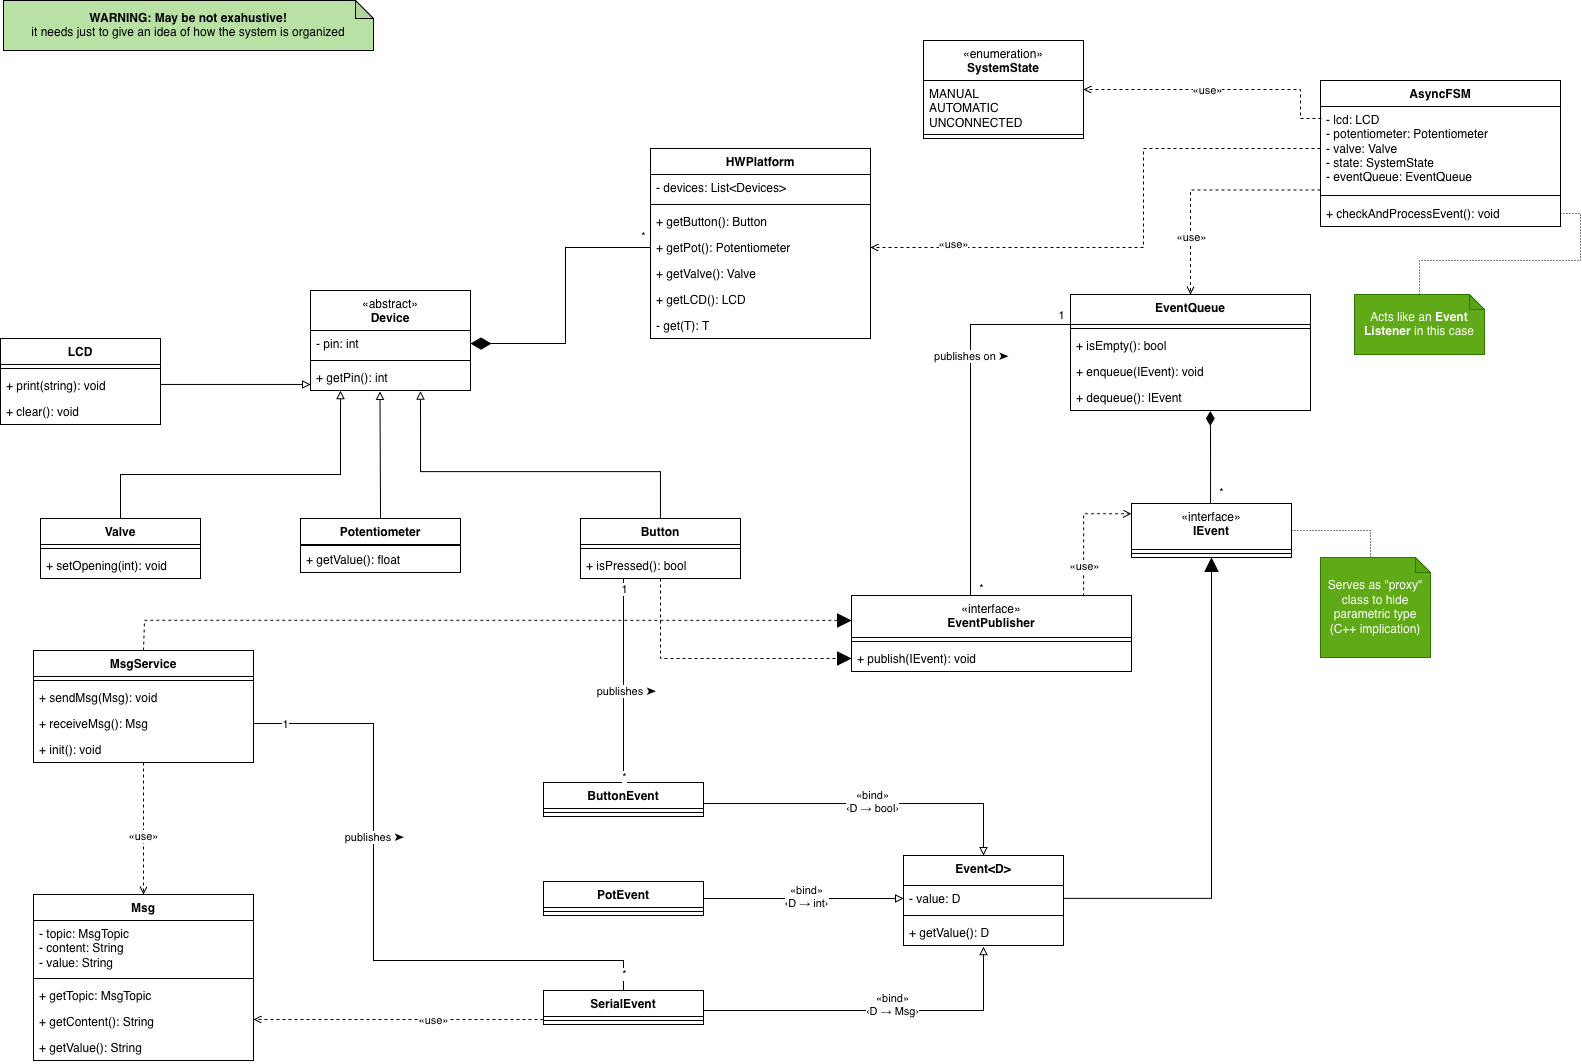
\includegraphics[width=\linewidth]{assets/imgs/WCS-Class-Diagram.drawio.png}
\caption{Subsystem class diagram (may not be exhaustive!)}
\end{figure}

\section{Dashboard Subsystem - (DBS)}
The \textbf{Dashboard Subsystem (DBS)} represents the graphical interface of the project, designed to provide human operators with an overview of the state of the system and remote control capabilities. It communicates exclusively with the \textbf{Control Unit Subsystem (CUS)} via asynchronous HTTP requests. It includea a visual mapping of raw JSON data into a level chart and it manages the operational modes.
\subsection{Implementation}
The subsystem is implemented using standard web technologies: \textbf{HTML5}, \textbf{CSS} for a responsive and intuitive layout, and \textbf{JavaScript} for dynamic data fetching from the CUS' APIs.
It performs periodic polling of the "status" endpoint, allowing the interface to reflect the current state of the tank and the valve without requiring a page refresh. This ensures that the operator is always presented with a real-time "digital twin" of the physical system.

\section{Tank Monitoring Subsystem - (TMS)}

\begin{figure}[H]
\centering
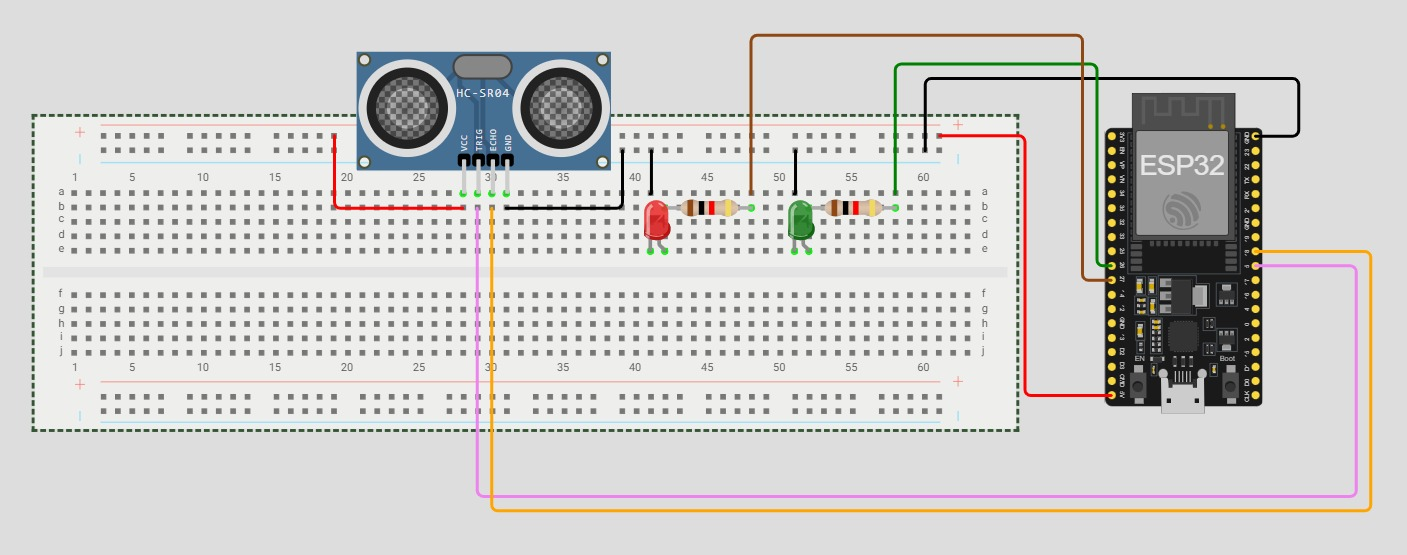
\includegraphics[width=\linewidth]{assets/imgs/TMS-Circuit.jpeg}
\caption{Subsystem circuit.}
\end{figure}

\begin{figure}[H]
\centering
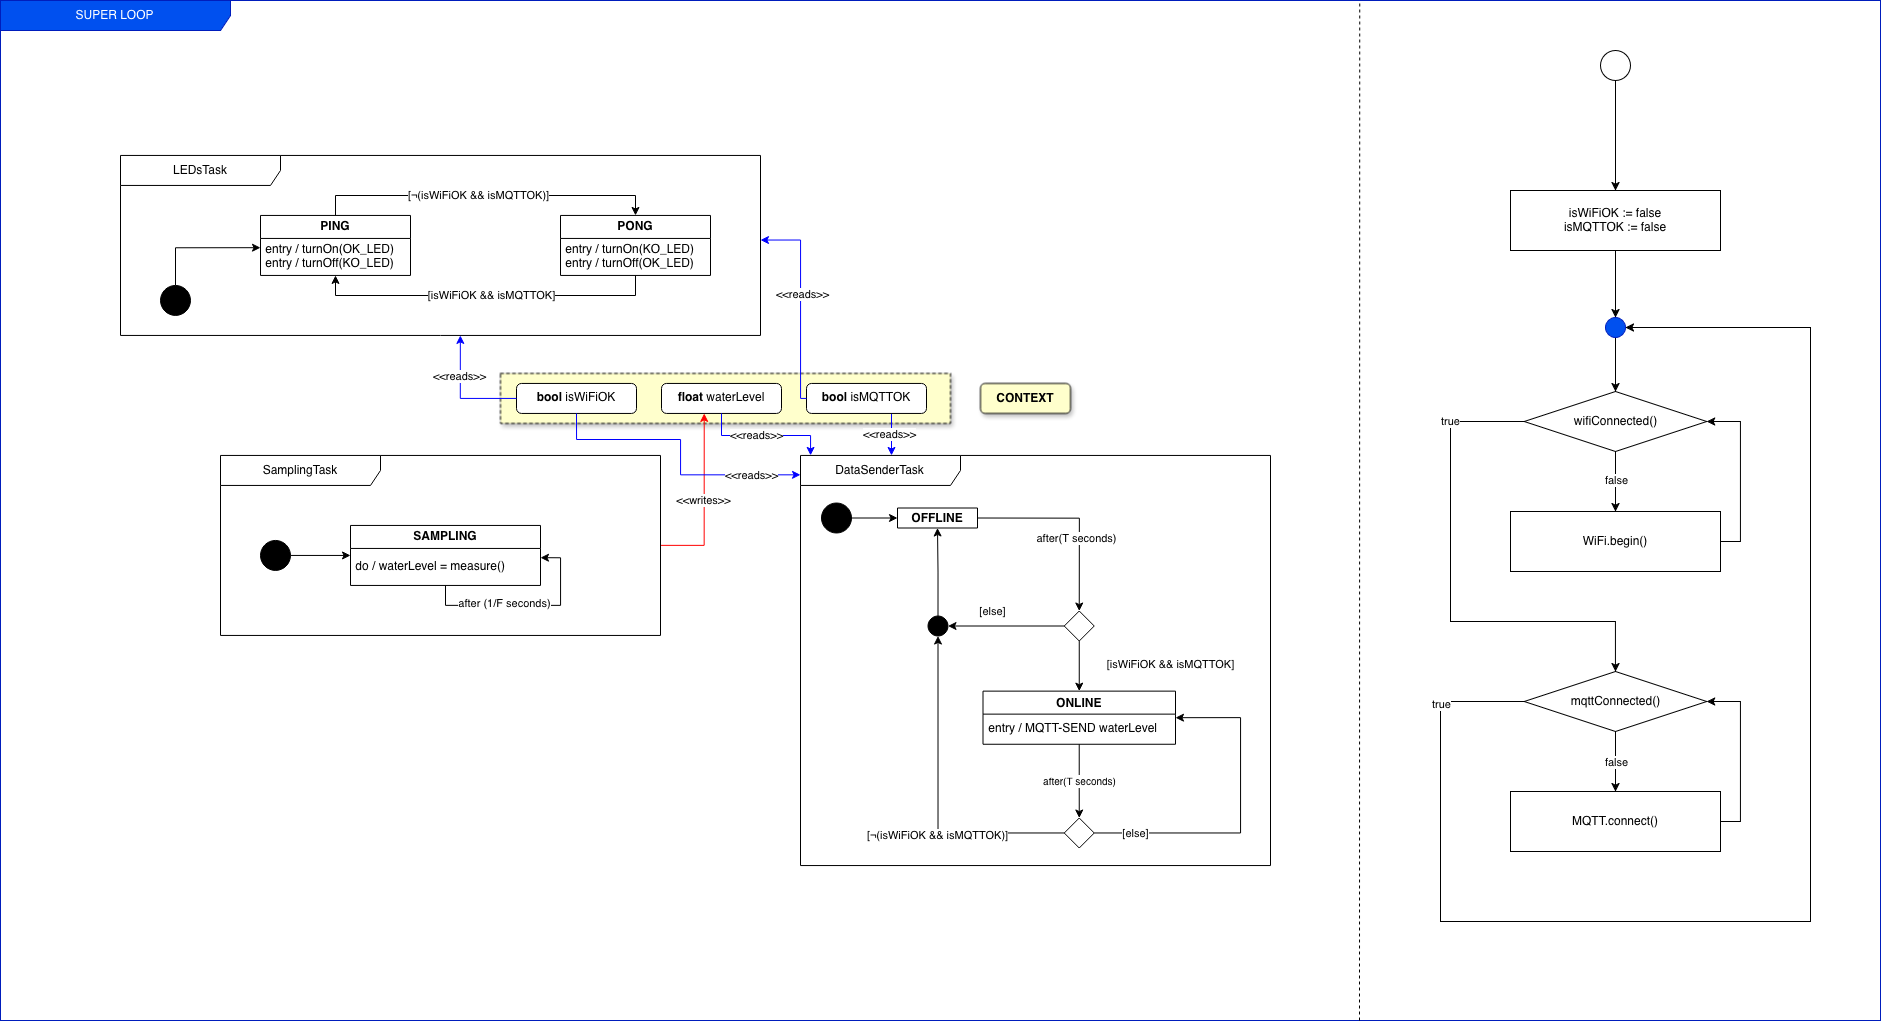
\includegraphics[width=\linewidth]{assets/imgs/TMS-Sync.drawio.png}
\caption{Subsystem synchronous FSM.}
\end{figure}

\subsection{Implementation}
The system requirements talk about data sampling carried out periodically, so we immediately thought that designing the system with a \textbf{Synchronous Finite State Machine} would carry out the task in the best way possible. We designed 3 main tasks, each briefly described as follows:
\begin{itemize}
    \item \verb|LEDsTask| is the task responsible for handling the LEDs according to the requirements - the KO Led is turned on when the system is disconnected (i.e. cannot reach MQTT Broker), otherwise is turned off (and the reverted logic applies to the OK Led);
    \item \verb|SamplingTask| constantly reads the sampled values from the Sonar sensor and stores them into a shared variable;
    \item \verb|DataSenderTask| reads the sampled values received from the \verb|SamplingTask| and, if there's an estabilished connection, sends them via MQTT to the broker. 
\end{itemize}

The connection of the whole subsystem is managed directly inside the superloop because we thought it as an asynchronous operation: at any point in time disconnection can happen, and therefore the system status must be updated almost in real-time.  

\label{sec:conc}

% Uncomment following to add an acknowledgement section
% \section*{Acknowledgements}

% Thanks again to \textbf{Person 1} and \textbf{Affiliation A} for their financial support.

% ----------
% Bibliography
% ----------

% Uncomment the following and add your references into biblio.bib file
% \bibliography{./biblio.bib}
% \bibliographystyle{abbrv}

\end{document}

% ----------
